\section{Heurística Constructiva Golosa}

\subsection{Algoritmo}
Para el desarrollo de este algoritmo partimos analizando las características de la soluci\'on que se quiere obtener. 
Como se busca un coloreo de máximo impacto posible, comenzamos considerando un coloreo de los nodos que sea seguro es de m\'aximo imapco, aunque no sea necesariamente un coloreo válido de G: aquella que surge de pintar todos los nodos con el mismo color (este coloreo solamente es un v\'alido para el grafo G si \'este solo cuenta con nodos aislados). 

La idea es partir de este coloreo de m\'aximo impacto en H y proceder modificando el color de la menor cantidad de nodos posible hasta que se halle un coloreo válido para G, momento en el cual se deja de iterar y se devuelve el coloreo obtenido en ese momento. Qué nodo se priorizar\'a modificar en cada paso se define en base a los siguientes criterios:

\begin{enumerate}
	\item Deberá ser un nodo que no se haya modificado en algún paso anterior del algoritmo.
	\item Modificar el nodo disminuye lo menos posible el impacto que obtenido hasta ese momento; es decir, es un nodo cuyo aporte al impacto es el menor posible.
\end{enumerate}

En caso de que dos o más nodos cumplan ambos puntos (lo que querría decir que modificar el color de cualquiera de ellos disminuye en la misma cantidad el impacto, y que esa cantidad es la menor que se podría disminuir), definimos los siguientes criterios de desempate: 

\begin{enumerate}
	\item Elegir al nodo que tenga mayor grado en G (ya que se busca lograr un coloreo legal de G modificando la menor cantidad de nodos posibles y al tener el nodo una mayor cantidad de vecinos en G modificar su color podría acercarnos más a un coloreo válido de G). 
	\item Si se produce un nuevo empate, elegir al nodo que tenga menor grado en H (porque se busca maximizar el impacto).
\end{enumerate}

A la hora de implementar esto, sin embargo, a\~nadimos un idea m\'as. Como precisábamos un algoritmo goloso con cierto grado de aleatoriedad, definimos un par\'ametro $porcentaje$, un número real entre 0 y 1, usado de la siguiente manera:
el proceso de elección del nodo anteriormente mencionado se implementó ordenando una lista de posibles nodos a modificar de manera tal que el nodo que mejor se ajuste a los requerimientos se encuentre en la primera posición. Una vez ordenada esta lista, elegimos el nodo que se corresponda con el índice (dentro de dicha lista) que se obtiene a partir de un número pseudoaleatorio, calculando el resto de dividirlo por el porcentaje $porcentaje$ del tamaño de la lista más 1 (es decir, índice = rand() \% lista.size() * $porcentaje$ + 1). Es fácil observar que si $porcentaje$=0, entonces se devolverá el primer elemento de la lista, que es el nodo que mejor se ajusta a los criterios de elección. \\

\indent La función que se encarga de la elección del nodo es $siguienteModificable$, que será llamada por $maximoImpactoGoloso$ hasta que se encuentre un coloreo válido. $maximoImpactoGoloso$ es además la encargada de aplicar el cambio de color en el nodo devuelto por $siguienteModificable$.\\

\indent El pseudocódigo es el que siguiente:\\

%\quad Analizando las características del problema implementamos una heurística constructiva golosa con los siguientes objetivos:

%\quad

%\quad \quad \quad - Empezar con el impacto máximo posible (cantidad de aristas de H)

%\quad 

%\quad \quad \quad - Modificar la menor cantidad de nodos posibles

%\quad

%\quad \quad \quad - El nodo que se modifique, tendría que bajar lo menos posible el impacto

%\quad En \textit{maximoImpactoGoloso} primero se colorea a todos los nodos con el mismo color, por lo que, sin tener en cuenta al grafo G, el impacto en H es máximo. Mientras que no sea legal este coloreo en G, se va a ir modificando los nodos. Apenas se consiga un coloreo legal se detiene. Por lo tanto, no necesariamente el ciclo principal itera la cantidad de nodos (en el peor caso sí).

%\quad En \textit{siguienteModificable} se obtiene el nodo a modificar. Se crea una lista de nodos que no hayan sido modificados y se calcula para cada uno su aporte al impacto en H. Se ordena la lista por los siguientes criterios:

%\quad

%\quad \quad - Menor impacto en H aportado: se desea modificar al que menos aporta para ver si cambiando de color aporta más.

%\quad

%\quad \quad - Mayor grado en G: se busca que cuanto antes el coloreo de G sea legal modificando lo menos posible, y modificando un nodo de grado grande se podria conseguir esto.

%\quad 

%\quad \quad - Menor grado en H: por lo que dijimos, en caso de empate de los anteriores criterios, queremos modificar lo menos posible en G y H

%\quad Pseudocódigo:

\begin{algorithm}[H]
\caption{} 
\begin{codebox}
\Procname{$\proc{maximoImpactoGoloso}(Grafo$ g$, Grafo$ h$, double porcentaje)$}

\li vector$<$unsigned int$>$ $res(n+1)$
\li int $solucion[0] \gets 0$
\li vector$<$unsigned int$>$ $coloreo(n,1)$
\li vector$<$bool$>$ $modificados(n,false)$
\li \While not G.coloreoLegal(coloreo)) \Do
\li nodo $ \gets $ siguienteModificable(G,H,modificados,porcentaje)
\li \For c desde 1 hasta colores.size() \Do
\li \If G.colorLegalDelNodo(nodo,coloreo,c)
\li coloreo$ [nodo] \gets $ c
\li exitFor
\End
\End
\End
\li $solucion[0] \gets$ impacto(h, coloreo)
\li \For i desde 0 hasta n \Do
		\li $solucion[i+1]=coloreo[i]$
	\End
\li	return $solucion$
\End
\end{codebox}
\end{algorithm}


\begin{algorithm}[H]
\caption{} 
\begin{codebox}
\Procname{$\proc{siguienteModificable}(Grafo$ g$, Grafo$ h,vector$<$bool$>$ modificados, double porcentaje)}

\li vector$<$pair$<$ unsigned int, unsigned int $>$ $>$ posibles
\li \For n nodo in V(G) \Do
\li \If not modificados$ [ $ nodo $ ] $
\li    agregar(posibles,$<$G.impactoNodo(nodo,H,coloreo),nodo$>$)
\End
\End
\li
\li sort(posibles)
\li
\li unsigned int res $ \gets $ random($ \vert $ posibles  $ \vert $ * porcentaje)
\li
\li return res
\End
\end{codebox}
\end{algorithm}

\quad


\subsection{Análisis de complejidad}

\indent Comencemos analizando la complejidad de la función impactoNodo.\\
\indent Esta función mira para un nodo el impacto que aporta en H, comparando su color con el de sus vecinos. Dicho nodo tiene en H a lo sumo n-1 vecinos. Luego, impactoNodo cuesta O(n).

\indent Analicemos ahora siguienteModificable. Al inicio comienza iterando sobre la cantidad de nodos de H y si dicho nodo no fue modificado o si no tiene vecinos, se calcula el impacto de cada nodo y se lo agrega a un vector de nodos candidatos a ser modificados.En el peor caso, todos los nodos están sin modificar y tienen vecinos,por lo tanto esto cuesta O($n^{2}$).\\
\indent Luego, se ordena de manera creciente el vector de candidatos de acuerdo al impacto de cada nodo.En el peor caso dicho vector tiene n elementos, pues todos los nodos son modificables y ordenarlos cuesta entonces O(n*log(n)).\\
\indent Luego, se itera sobre la cantidad de elementos de ese vector, esta vez para desempatar los nodos. En el peor caso todos los nodos empatan en el impacto que generan. Desempatarlos a todos cuesta en el peor caso O($n^{2}$) , que el caso en el que se invirtió el orden del vector por desempates.\\
\indent A continuación se elige pseudoaleatoriamente en O(1) uno de los primeros elementos del vector.\\
\indent Pasando en limpio, siguienteModificable cuesta O($n^2$ + n*log(n)+ $n^2$), que es O($n^{2}$).\\

\indent Ahora analicemos maximoImpactoGoloso.\\
\indent Al principio realiza unas cuantas operaciones en O(n). De estas es destacable la creación de un vector de tamaño igual al grado del nodo con grado máximo de G, que refiere a la cantidad de colores a usar. Pero el grado máximo de cada nodo es a lo sumo n-1. Luego crear ese vector cuesta O(n).\\
\indent Luego, se ejecuta un while que a lo sumo itera n veces. Esto es porque en el peor caso tuve que pintar todos los nodos de distinto color hasta obtener un coloreo válido.\\
\indent Dentro de ese while está implícito el chequeo de si el coloreo es válido, que cuesta O(n+m), donde vamos a acotar a m como el máximo entre las aristas de G y de H. Se ejecuta siguienteModificable y se itera luego en la cantidad de colores, costando cada iteración en la cantidad de colores O(n) que es lo que cuesta ver si pintar un nodo de ese color es no coincide con el color de uno de los vecinos de ese nodo, que como mencionamos antes pueden ser n-1.\\
\indent Luego, lo de adentro del while cuesta O(n+m+ $n^{2}$) y el costo total del while es de O(n(n+m +$n^{2}$)), que es O(n*(n+m)+ $n^{3}$).\\
\indent Luego de iterar se calcula el impacto de dicho coloreo en O(n+m).\\
\indent Es decir que en total maximoImpactoGoloso cuesta O(n+n*(n+m)+ $n^{3}$ + n+m).\\
\indent Por lo tanto, maximoImpactoGoloso cuesta O(n*(n+m)+ $n^{3}$).\\
 
\subsection{Experimentación y Resultados}


\subsubsection{Optimización del parámetro}

\quad Como explicamos anteriormente, nuestra heurística recibe un parámetro que determina la aleatoriedad de la elección del siguente nodo a colorear con el objetivo de encontrar un coloreo del grafo G válido.

\quad Comparamos los resultados obtenidos por el goloso contra la metaheurística GRASP, y calculamos la distancia de las soluciones. Es decir, la diferencia entre ambas. Probamos con 50, 100, 150 y 200 nodos con 100 repeticiones por cada cantidad de nodos. Testeamos con grafos aleatorios por su diversidad en tipos de grafos. Calculando un promedio obtuvimos:

\begin{figure}[H]
	\centering
	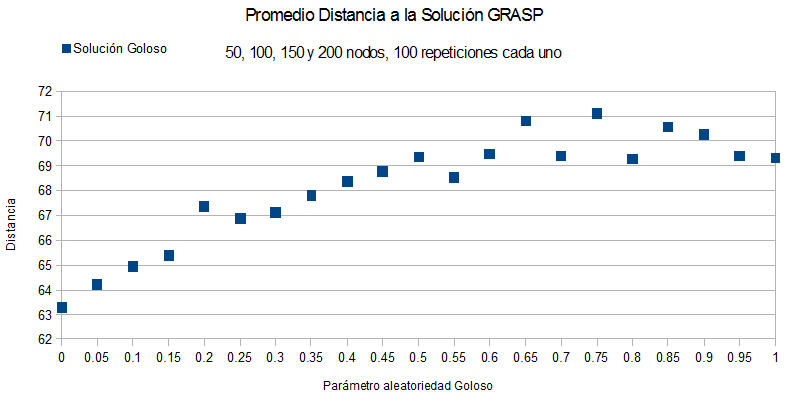
\includegraphics[scale=0.6]{optimizacionGoloso.png}
\end{figure}

\quad Podemos observar que cuanto mayor sea la cantidad de nodos a elegir aleatoriamente empeora el resultado. Esto se debe a que en la porción de lista que elegimos al azar, se encuentra ordenada por los criterios anteriormente desarrollados. Con lo que al principio se encuentran los mejores candidatos. Concluimos con que si se utiliza solamente esta heurística, es conveniente que el valor del parámetro sea 0.

\subsubsection{Costo temporal}

\quad Una vez analizado el tema del parametro vamos a tomar el costo temporal de la heurística.

\quad Analizaremos con grafos del tipo aleatorio, grafos de forma estrella no uniforme y grafos de red de 4 vértices.

\begin{figure}[H]
	\centering
	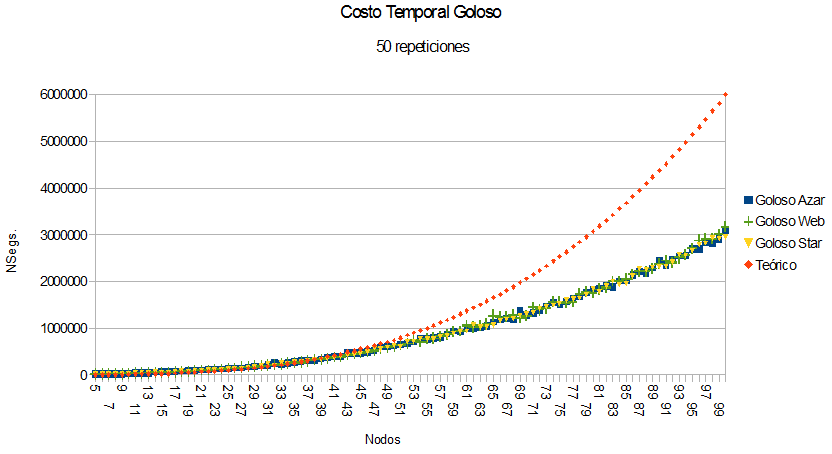
\includegraphics[scale=0.6]{timingGoloso.png}
\end{figure}

\quad

\quad Podemos observar que efectivamente se cumple con la cota teórica calculada anteriormente. Mantiene la tendencia asintótica de O($ n^{3}$) pero más \textit{suave}. 

\quad Si comparamos con las gráficas obtenidas con el método exacto es drástico la mejora en cuanto costos temporal pero como veremos más adelante lo que se gana en tiempo se pierde mucho en calidad de solución obtenida.

\quad Se observa que con las tres familias de grafos con las que testeamos no hay diferencias apreciables en cuanto a costo temporal.